\subsection{Terrain Generation Algorithms}
Terrain generation is essentially to generate a height for each point in 2D space. It can be seen as using a function to map \textit{x} and \textit{y} coordinates into \textit{z} coordinates: \[z=terrainGen(x, y)\]

In this project, we implemented three terrain generation algorithms, namely, Perlin Noise, Simplex Noise and Diamond Square. This section gives an overview of the three algorithms.

\subsubsection{Perlin Noise}
Perlin noise is procedurally generated noise proposed by Ken Perlin \cite{perlin:2002}. In 2D space, Perlin Noise works as follows:
\begin{enumerate}
	\item Create a grid of vectors, whose \textit{x} and \textit{y} coordinates are all integers. Every point in the 2D space falls into a square in the grid, where four vertexes of the square can be decided by taking the floors and ceilings of its \textit{x} and \textit{y} coordinates.
	\item For each vector on the grid, generate a gradient pointing away from it in a random direction (Figure~\ref{fig:randomGradients}).
	\item For any given point, interpolate the value from the surrounding 4 gradients.
	\item Sum all values of the interpolations. Some example graphs generated by Perlin noise are show in Figure~\ref{fig:perlinEg}.
\end{enumerate}
\begin{figure}
	\center
	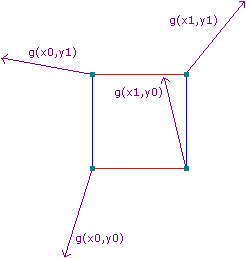
\includegraphics[scale=0.5]{images/gradients.png}
	\caption{Random Gradients}
	\label{fig:randomGradients}
\end{figure}
\begin{figure}
	\center
	\subfigure{
		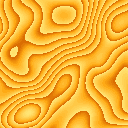
\includegraphics[scale=0.5]{images/woodgrain.png}
	}
	\subfigure{
		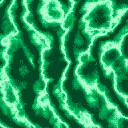
\includegraphics[scale=0.5]{images/marble.png}
	}
	\subfigure{
		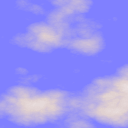
\includegraphics[scale=0.5]{images/clouds.png}
	}
	\caption{Perlin Noise Examples}
	\label{fig:perlinEg}
\end{figure}

\subsubsection{Simplex Noise}
Simplex noise is another noise generation algorithm developed by Perlin \cite{perlin:2001}. It makes the noise generation simpler and faster, in order to implement it on hardware. In 2D space, simplex noise differs from Perlin noise in the following ways:
\begin{enumerate}
	\item It uses a grid consists of equilateral triangles instead of squares. As a result, there are only three adjacent grid points for each point in the space.
	\item Summation is used instead of interpolation. Simplex noise sums up the contributions from each corner (grid point) of the triangle, where ``the contribution is a multiplication of the extrapolation of the gradient ramp and a radially symmetric attenuation function" \cite{Gustavson2005}. The calculation of summation is much less than interpolation, making simplex noise faster.
\end{enumerate}

\subsubsection{Diamond-Square}
Diamond-square algorithm is another method to generate height map of a terrain. It is different from above-mentioned algorithms in that it uses fractals. It works on a 2-dimension array of points; the number of points in each dimension should be a power of two, plus one (e.g. $17 \times 17$, $1025 \times 1025$, etc). The algorithm starts by assigning seed values as heights to the four corners of the square, then it starts its iterative subdivision routine in two steps:
\begin{itemize}
	\item \textbf{The diamond step} Average the heights of the four corners, add it to a random value and assign the sum as the height of the square \textit{midpoint}, where two diagonals meet. The midpoints and corners form diamond shapes in the grid.
	\item \textbf{The square step} Take each diamond of four points, average the heights of them and add it to a random value in the same range of previous step to get the sum. Assign the sum to the midpoint of the diamond as height. Once this done, it gives smaller squares again.
\end{itemize}
The iteration can repeat until all points in the grid have heights (Figure~\ref{fig:dsa}).
\begin{figure}
	\center
	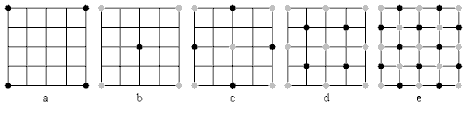
\includegraphics[scale=0.5]{images/dsa.png}
	\caption{Diamond-square Algorithm}
	\label{fig:dsa}
\end{figure}

\subsubsection{Combination of Algorithms}
Since all of the three algorithms accept \textit{x} and \textit{y} coordinates, and produce a height, we can combine these algorithms in different ways:
\begin{enumerate}
	\item Add up the height maps generated by several run of the same algorithm
	\item Add up the height maps of different algorithms
\end{enumerate}

By combining the algorithms, we are able to produce more different terrains than single algorithms.

% subsection algorithms (end)